\chapter{Elastyczne indeksowanie}

Termin ``elastyczne indeksowanie'' (\emph{flexible indexing}) określa nowe podejście do architektury Lucene, wprowadzone w wersji 4.0. Polega ono na oddzieleniu formatu indeksu (fizycznego sposobu zapisu poszczególnych jego elementów na dysku) od logicznych operacji na nim wykonywanych.

\section{Cel wprowadzenia zmian}

W październiku 2012 roku, po ok. dwóch latach prac, została opublikowana wersja 4.0 Lucene, znacząco różniąca się od poprzednich -- głównie dzięki wprowadzeniu tzw. \emph{architektury kodekowej}. Części biblioteki odpowiedzialne za indeksowanie zostały logicznie wydzielone i umieszczone w dodatkowej warstwie architektury (kodeku). 

Głównym powodem wprowadzenia zmian był przestarzały i nieelastyczny format kodowania indeksu. Wersje 3.x Lucene oraz wcześniejsze do zapisu list postingowych posługiwały się formatem \texttt{vInt} -- liczb całkowitych o zmiennej długości bitowej. Format ten był ściśle związany z wszystkimi częściami kodu. W związku z tym jakakolwiek jego modyfikacja wymagała sporego nakładu pracy programisty. Utrudniało to rozwój Lucene oraz eksperymentowanie z nowymi sposobami kompresji czy strukturami danych. Format \texttt{vInt} istniał w Lucene praktycznie od jej początków (ok. 10 lat, od wersji 1.0). Od tego czasu powstały efektywniejsze algorytmy kompresji.

Stara architektura uniemożliwiała także zapis dodatkowych statystyk do indeksu -- co utrudniało (lub uniemożliwiało) implementacje nowych algorytmów obliczania miar dopasowania dokumentu do zapytania.

Lucene, pomimo, że była najpopularniejszym narzędziem do wyszukiwania tekstowego stosowanym w komercyjnych projektach, rzadko była wykorzystywana w środowiskach naukowych -- właśnie ze względu na brak możliwości łatwych zmian formatów indeksu i eksperymentowania na nim. Nowa architektura miała to zmienić: umożliwić bardziej elastyczny rozwój przy jednoczesnym zachowaniu wydajności.

\section{Architektura oparta o kodeki}

Zmiany architektury polegały na wprowadzeniu dodatkowej warstwy pośredniczącej pomiędzy formatem dyskowym indeksu a biblioteką. Ilustruje to rysunek ~\ref{newarchitecture} (źródło: \cite{flexindex}).

\begin{figure}[here]
 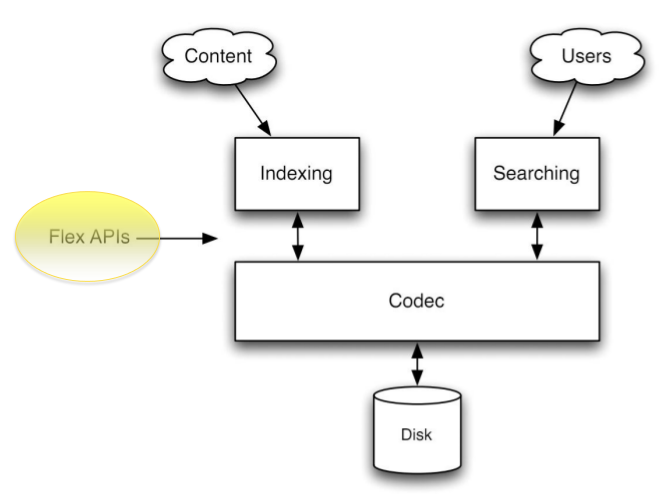
\includegraphics[scale=0.5]{architecture.png}
 \caption{Schemat architektury opartej o kodeki.}
 \label{newarchitecture}
\end{figure}

Operacje na indeksie (dodawanie, usuwanie lub modyfikowanie dokumentów, wyszukiwanie) są implementowane w wyższych warstwach biblioteki. Kodek dostarcza formatu narzędzi do zapisu i odczytu danych o zaindeksowanych dokumentach. Poprzez jego podmianę można zastosować np. niestandardowe algorytmy kompresji, struktury danych do przechowywania słowników termów itp.

\section{Struktura kodeka}

Każdy kodek składa się z ośmiu części. Istnieje możliwość łączenia istniejących rozwiązań z własnymi implementacjami. Oznacza to, że można skorzystać z domyślnych implementacji większości tych elementów i podmienić np. tylko część odpowiedzialną za kodowanie list postingowych.

Elementy, na które składa się kodek to:
\begin{enumerate}
 \item format list postingowych,
 \item format DocValues,
 \item format pól przechowywanych (\emph{stored fields}),
 \item format dla \emph{term vectors},
 \item format informacji o polach i związanych z tym statystyk (\emph{field infos format}),
 \item format zapisu ogólnych informacji dotyczących segmentów (\emph{segment info format}),
 \item format zapisu norm -- związanych z poszczególnymi polami liczb wskazujących, czy dane pole powinno być traktowane jako mniej lub bardziej istotne niż pozostałe (wskaźniki \emph{boost} zapisywanie podczas indeksowania),
 \item format do zapisu informacji o tym, które dokumenty powinny zostać usunięte podczas najbliższej optymalizacji indeksu (\emph{live docs format}).
\end{enumerate}
